\documentclass{article}
\usepackage{minted}
\usepackage{graphicx}
\begin{document}
\begin{minted}{python}
NAME:- J.suryateja
ID:-B192653
CLASS:- CSE C5
import pandas as pd
df=pd.read_csv("iris.csv")
import matplotlib.pyplot as pg
v=df['variety'].value_counts()
v=dict(v)
k=['iris setosa', 'iris versicolor','iris virginica']
j=v.values()
fig=pg.figure(figsize=(10,10))
pg.pie(x=j,labels=k, explode=[0.1,0.1,0.1],autopct='%1.1f%%',shadow=True,)
pg.title('iris.species%')

pg.legend()
pg.show()
import itertools
l1=df['sepal.length']
l2=df['variety']
l3=df['sepal.width']
setosal=[]
setosaw=[]
Virginical=[]
Virginicaw=[]
Versicolorl=[]
Versicolorw=[]


for (i,j,k) in zip(l1,l2,l3):
    if j=="Setosa":
        setosal.append(i)
        setosaw.append(k)
    elif j=="Virginica":
        Virginical.append(i)
        Virginicaw.append(k)
    else:
        Versicolorl.append(i)
        Versicolorw.append(k)
#print(setosal)
#print(Versicolorl)
#print(Virginical)
fig=pg.figure(figsize=(7,5))
pg.title("The Iris Data Set")
u=pg.scatter(setosal,setosaw,color='red')
v=pg.scatter(Virginical,Virginicaw,color='blue')
z=pg.scatter(Versicolorl,Versicolorw,color='green')
pg.ylabel('sepal.width')
pg.xlabel('sepal.length')
pg.grid(linestyle = '--')
pg.legend([u,v,z], ['Setosa','Virginica','Versicolor'])
pg.show()
import itertools
l1=df['petal.length']
l2=df['variety']
l3=df['petal.width']
setosapl=[]
setosapw=[]
Virginicapl=[]
Virginicapw=[]
Versicolorpl=[]
Versicolorpw=[]


for (i,j,k) in zip(l1,l2,l3):
    if j=="Setosa":
        setosapl.append(i)
        setosapw.append(k)
    elif j=="Virginica":
        Virginicapl.append(i)
        Virginicapw.append(k)
    else:
        Versicolorpl.append(i)
        Versicolorpw.append(k)
#print(setosapl)
#print(Versicolorpl)
#print(Virginicapl)
y=['sepal.length','sepal.width','petal.length','petal.width']
x=["Setosa","Virgincia","Versicolor"]
df2=df.groupby('variety').agg('mean')
df2.head()


df2.T.plot(kind='bar')

pg.xticks(rotation='horizontal')
pg.legend(loc='center left', bbox_to_anchor=(1, 0.85))
pg.xlabel("Features")
pg.ylabel('value in cm')
fig=pg.figure(figsize=(10,8))
pg.title("Iris Histograms")
pg.subplot(2,2,1)
pg.hist(df['sepal.length'])
pg.xlabel('sepal length(cm)')
pg.ylabel('Frequency')
#pg.tight_layout() 
pg.subplot(2,2,2)
pg.hist(df['sepal.width'],color = "orange")
pg.xlabel('sepal width(cm)')
pg.ylabel('Frequency')
pg.subplot(2,2,3)
pg.hist(df['petal.length'],color = "Green")
pg.xlabel('petal length(cm)')
pg.ylabel('Frequency')
pg.subplot(2,2,4)
pg.hist(df['petal.width'],color = "Red")
pg.xlabel('petal width(cm)')
pg.ylabel('Frequency')
\end{minted}
\begin{figure}[htbp]
\centerline{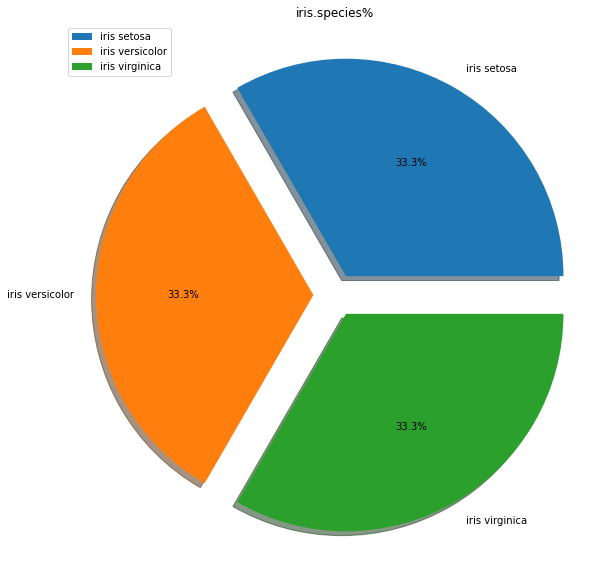
\includegraphics[width=5in, height=5in,]{pie.png}}
\centerline{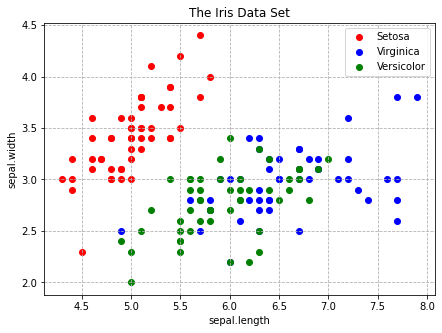
\includegraphics[width=4in, height=4in,]{scatterplot.png}}

\end{figure}
\newpage
\begin{figure}[htbp]
\centerline{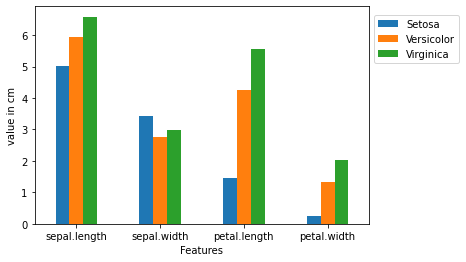
\includegraphics[width=5in, height=5in,]{bar.png}}
\centerline{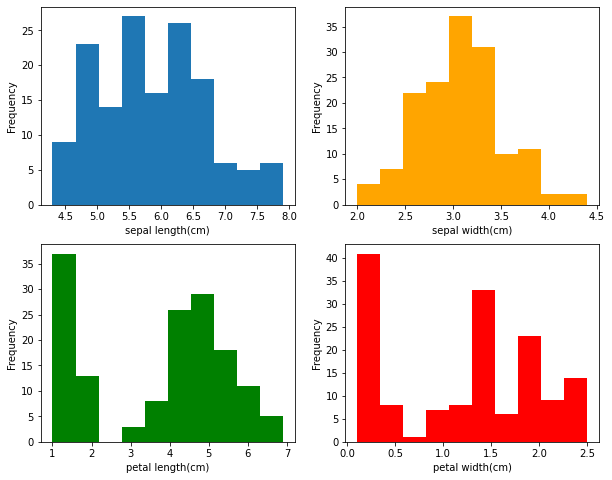
\includegraphics[width=5in, height=5in,]{hist.png}}

\end{figure}
\end{document}
